\chapter{Risultati e discussione}
\label{cap:risultati}

Il capitolo presenta gli esiti della pipeline distinguendo le prove storiche riportate nella matrice di accettazione dagli artefatti conservati del ciclo V4. Le prime documentano la copertura integrale dei tre profili; sui secondi si basa l'analisi di due esecuzioni selettive, dei loro elementi e delle 17 richieste di captioning. Come introdotto nel Capitolo~\ref{cap:metodi}, la copertura dei manuali completi e l'accettazione delle versioni precedenti restano riferite alle prove storiche, mentre i campioni finali descrivono il nuovo setup.

Per valutare la qualità della rappresentazione, si confrontano puntualmente i ritagli, i testi acquisiti e le risposte conservate. Questa analisi è distinta dalle schede qualitative richiamate nel diario, assenti dall'archivio del progetto, e resta circoscritta agli esempi discussi, senza un'annotazione indipendente dell'intero corpus. Gli esempi rendono verificabili aggiunte informative, errori e limiti dei controlli; la valutazione resta descrittiva, senza un punteggio generale di qualità.

\section{Esiti della pipeline integrata per profilo}
\label{sec:risultati-struttura}

\subsection{Copertura integrale documentata}

La matrice di accettazione riporta la produzione di una rappresentazione gerarchica per ciascuno dei tre profili. La Tabella~\ref{tab:risultati-storici} sintetizza le prove complete dello schema 1.0, mantenendole separate dai risultati successivi dello schema 1.1.\footnote{\raggedright \path{tesi-di-nardo/docs/acceptance-matrix.md}, sezione ``Evidenza storica per profilo --- schema 1.0''. Per il digitale con outline la run è \path{case1-full-no-enrich-20260712c}; per quello ricostruito \path{case2-full-no-enrich-20260712b}; il caso OCR è documentato mediante esecuzione reale e replay delle risposte dei worker. I relativi bundle integrali non sono inclusi nell'archivio del progetto.}

\begin{table}[!htbp]
\centering
\caption{Esiti integrali dello schema 1.0 dalla matrice storica, non da nuove esecuzioni. Le prove senza enrichment, incluso il replay OCR, superano i 29 controlli dello schema ma non il gate dell'enrichment.}
\label{tab:risultati-storici}
\small
\begin{tabularx}{\textwidth}{@{}>{\raggedright\arraybackslash}Xrrrr@{}}
\toprule
Profilo & \shortstack{Pagine\\elaborate/totali} & Capitoli & Elementi & Asset \tabularnewline
\midrule
Digitale con outline & 1112/1112 & 963 & 14.047 & 2355 \\
Digitale ricostruito & 1112/1112 & 958 & 14.047 & 2355 \\
Scansione OCR & 34/34 & 15 & 350 & 65 \\
\bottomrule
\end{tabularx}
\end{table}

I due PDF digitali producono lo stesso numero di elementi e asset, ma non la stessa TOC. Questo è coerente con l'uso dello stesso parser dei contenuti e di due strategie strutturali diverse sul medesimo manuale di base. I conteggi indicano che il cambiamento del percorso strutturale ha lasciato invariata la consistenza quantitativa dell'acquisizione riportata; l'identità semantica degli elementi e la correttezza delle associazioni richiedono invece un confronto dei contenuti.

Per il profilo ricostruito la matrice registra 958 voci contro i 963 segnalibri della variante originale. Riporta inoltre un confronto su titoli, pagine, ordine e livelli; tuttavia, l'assenza dell'harness e delle corrispondenze elementari non permette di ricalcolarlo. Anche i riepiloghi dei titoli corrispondenti e di quelli mancanti o extra richiederebbero il dettaglio delle regole di abbinamento per essere riconciliati. Le differenze non vengono quindi trasformate qui in una nuova stima di precision o recall.

Nel caso scansionato, la prova completa documenta un indice individuato a pagina 5, uno scarto di numerazione pari a una pagina e 15 riferimenti risolti su 15. La matrice riferisce anche l'ispezione dei ritagli delle pagine 26 e 33, acquisite con orientamento a 180 gradi. Questi risultati sostengono l'accettazione del percorso sul WM250 considerato, non su qualunque scansione o impaginazione.

\subsection{Esiti delle esecuzioni del ciclo V4}

Le due run V4 del 15 settembre 2026 terminano con codice di uscita zero e pubblicano un bundle. Entrambi i manifest dichiarano \texttt{experimental}, mentre entrambi i report salvati riportano \texttt{passed} con 30 controlli superati. La Tabella~\ref{tab:risultati-v4} riassume la rappresentazione ottenuta.\footnote{Dati ricavati da \path{bundle/run.json}, \path{bundle/manual.json}, \path{bundle/validation.json} e \path{evidence/outcome.json} nei casi \texttt{outline} e \texttt{scanned} di \path{tesi-di-nardo/enrichment-v4-final-20260915}.}

\begin{table}[!htbp]
\centering
\caption{Bundle selettivi V4, entrambi sperimentali. I capitoli non rientrano negli elementi: l'outline digitale copre l'intero PDF, la struttura OCR le sole pagine selezionate. Le caption conservate includono quelle da rivedere.}
\label{tab:risultati-v4}
\small
\begin{tabularx}{\textwidth}{@{}Xrr@{}}
\toprule
Indicatore & Digitale con outline & Scansione OCR \\
\midrule
Pagine elaborate / totali & 6/1112 & 4/34 \\
Pagine con elementi / elaborate & 6/6 & 4/4 \tabularnewline
Capitoli e voci TOC disponibili & 963 & 10 \tabularnewline
Elementi canonici & 70 & 47 \\
Elementi di testo & 39 & 24 \\
Elementi titolo & 15 & 14 \\
Immagini & 16 & 9 \\
Tabelle & 0 & 0 \\
Caption conservate nel documento & 8 & 5 \\
Controlli superati / previsti & 30/30 & 30/30 \tabularnewline
\bottomrule
\end{tabularx}
\end{table}

Nel digitale la presenza di 963 capitoli non significa che tutte le sezioni siano state elaborate: l'outline è acquisito dall'intero PDF, mentre il contenuto è limitato alle sei pagine richieste. Nello scansionato la struttura deriva invece dalle sole quattro pagine selezionate. Poiché l'indice stampato a pagina 5 non è incluso, viene attivato il fallback sui titoli OCR, che produce dieci capitoli. La differenza rispetto alle quindici voci della prova completa è quindi legata anche alla selezione delle pagine e non prova, da sola, un peggioramento del motore.

Le due esecuzioni mostrano la convergenza di parser e strutture differenti sullo stesso contratto \texttt{ManualDocument}. Gli artefatti prodotti confermano la coerenza dei file; la completezza semantica dell'intero manuale resta fuori dall'obiettivo di queste due run.

\subsection{Durate registrate}

Le registrazioni distinguono la durata dell'esecuzione complessiva da quella dell'enrichment. Nel caso digitale sono documentati circa 77,48 secondi per la CLI e 64,79 secondi per l'enrichment; nel caso OCR circa 480,47 e 58,74 secondi, rispettivamente. I valori provengono da \texttt{outcome.json} e dal \texttt{call.json} dello stadio di enrichment, non dalla differenza approssimata tra orari visualizzati.

Il tempo esterno all'enrichment comprende operazioni diverse, tra cui preparazione, parsing, rendering e controlli. Il maggiore tempo totale della selezione OCR non può essere attribuito al captioning, né trasformato in una graduatoria di velocità fra parser: cambiano documento, numero di pagine e lavoro svolto. Si tratta di due osservazioni operative senza repliche, non di misure medie di throughput.

La Figura~\ref{fig:durate-v4} separa visivamente l'enrichment dal resto del tempo CLI, mantenendo una scala comune e indicando i diversi carichi delle due selezioni.

\begin{figure}[!htbp]
\centering
\begin{tikzpicture}[schema base]
\foreach \secondi in {0,100,200,300,400,500} {
  \draw[draw=schemaGrigio!20,line width=0.4pt] ({3.4+0.021*\secondi},0) -- ({3.4+0.021*\secondi},-3.8);
  \node[schema nota] at ({3.4+0.021*\secondi},-4.15) {\secondi};
}
\node[schema etichetta,text width=2.8cm] at (1.55,-0.85) {\textbf{Digitale}\newline 6 pagine\newline 9 richieste};
\node[schema etichetta,text width=2.8cm] at (1.55,-2.8) {\textbf{Scansione}\newline 4 pagine\newline 8 richieste};
\path[draw=schemaBlu,fill=schemaCartaBlu] (3.4,-1.19) rectangle (4.760505,-0.51);
\path[draw=schemaGrigio,fill=schemaGrigio!18] (4.760505,-1.19) rectangle (5.027090,-0.51);
\node[schema nota,anchor=west] at (5.3,-0.85) {77,48 s};
\path[draw=schemaBlu,fill=schemaCartaBlu] (3.4,-3.14) rectangle (4.633537,-2.46);
\path[draw=schemaGrigio,fill=schemaGrigio!18] (4.633537,-3.14) rectangle (13.489805,-2.46);
\node[schema nota,anchor=south east] at (13.489805,-2.35) {480,47 s};
\draw[draw=schemaGrigio,line width=0.7pt] (3.4,-3.8) -- (13.9,-3.8);
\node[schema etichetta] at (8.65,-4.75) {Durata CLI (secondi)};
\path[draw=schemaBlu,fill=schemaCartaBlu] (0.3,-5.6) rectangle +(0.4,0.3);
\node[schema nota,anchor=west] at (0.85,-5.45) {Enrichment: 64,79 / 58,74 s};
\path[draw=schemaGrigio,fill=schemaGrigio!18] (7.6,-5.6) rectangle +(0.4,0.3);
\node[schema nota,anchor=west] at (8.15,-5.45) {Resto: 12,69 / 421,73 s};
\end{tikzpicture}
\caption{Durate delle due run V4, da \texttt{outcome.json} e dal \texttt{call.json} dell'enrichment. In legenda: digitale / scansione. Il resto è calcolato per differenza e non misura il solo OCR. Documenti e carichi diversi, senza repliche: il grafico non confronta la velocità dei parser.}
\label{fig:durate-v4}
\end{figure}

\section{Qualità della rappresentazione comune}
\label{sec:risultati-asset}

\subsection{Gerarchia coerente e associazioni non equivalenti}

I report V4 non segnalano identificativi duplicati o incoerenze dei riferimenti padre--figlio. Ciò non esclude associazioni documentali semanticamente troppo deboli. Un caso concreto compare nella pagina 10 del WM250: le tre immagini della pagina sono collocate nel capitolo \enquote{8. Cross Slide Lock}, mentre la prima è richiamata dai paragrafi relativi ai comandi A, B e C della Figura 11 e la seconda dai selettori D ed E della Figura 12.

Per \texttt{paddle-image-0010-0001}, il prompt effettivamente salvato usa i titoli \enquote{Emergency Button ON/OFF Switch}, \enquote{Change-over Switch} e \enquote{Variable Speed Control Switch}. Per \texttt{paddle-image-0010-0002} usa invece \enquote{Feed Direction Selector} e \enquote{Feed Rate Selector}. Il recupero del contesto tramite richiamo alla figura seleziona dunque sezioni più pertinenti rispetto al padre canonico.\footnote{Confronto tra \path{scanned/bundle/manual.json} e le richieste \path{scanned/evidence/captions/0004/call.json} e \path{scanned/evidence/captions/0005/call.json}, sotto l'archivio V4. I testi associati sono conservati anche nella snapshot precedente all'enrichment.}

Questo risultato mostra sia un recupero utile sia un limite: il contesto della richiesta viene corretto localmente, ma il riferimento gerarchico dell'immagine non viene aggiornato. Un utilizzatore del solo albero documentale riceverebbe ancora l'associazione al capitolo finale della pagina. Non si può quindi considerare risolto il problema dell'appartenenza solo perché il prompt usa informazioni pertinenti.

La Figura~\ref{fig:gerarchia-contesto-wm250} affianca il ritaglio originale alle due associazioni documentali, rendendo esplicito che il recupero del contesto non corregge automaticamente l'albero.

\begin{figure}[htbp]
\centering
\begin{tikzpicture}[schema base]
\node[schema titolo] at (0,0.3) {Stessa immagine, due associazioni documentali diverse};
\path[schema pannello] (0,-0.2) rectangle (5,-6.65);
\node[schema etichetta,text width=4.6cm] at (2.5,-0.7) {\textbf{WM250, pagina 10}\newline Figura 11 del manuale};
\node[inner sep=0] at (2.5,-3.4)
  {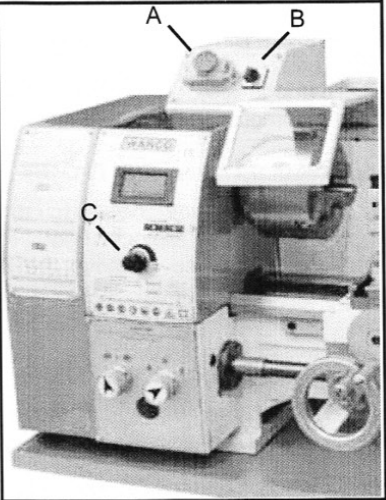
\includegraphics[width=3.1cm]{figure/asset/v4/paddle-image-0010-0001.png}};
\node[schema nota,text width=4.4cm] at (2.5,-6)
  {Asset originale};
\node[schema esterno,text width=7.7cm,minimum height=1.8cm] (padre) at (10.6,-1.45)
  {\textbf{Padre salvato in manual.json}\\\enquote{8. Cross Slide Lock}\\Associazione canonica non aggiornata};
\node[schema blocco,text width=7.7cm,minimum height=2.9cm] (contesto) at (10.6,-5)
  {\textbf{Contesto nella richiesta 0004}\\[4pt]
  A -- Emergency Button ON/OFF Switch\\
  B -- Change-over Switch\\
  C -- Variable Speed Control Switch\\[4pt]
  Sezioni che richiamano la Figura 11};
\draw[schema freccia,draw=schemaOcra] (5,-1.45) -- (padre.west);
\draw[schema freccia,draw=schemaBlu] (5,-5) -- (contesto.west);
\node[schema nota,text width=14.3cm] at (7.5,-7.45)
  {Il contesto della richiesta è più pertinente, ma il capitolo padre non viene corretto.};
\end{tikzpicture}
\caption{Due associazioni per \texttt{paddle-image-0010-0001}, da \texttt{manual.json} e dalla richiesta OCR \texttt{0004}. I richiami contestuali non sono nuovi capitoli. La discrepanza è ispezionabile anche se la caption viene esclusa per lunghezza.}
\label{fig:gerarchia-contesto-wm250}
\end{figure}

Anche le tavole delle pagine 26 e 33 rimangono sotto lo stesso capitolo, conseguenza della struttura parziale ottenuta senza l'indice. Nelle rispettive richieste capitolo e contesto locale sono però dichiarati non disponibili: il modello non riceve come argomento il titolo di una sezione lontana e non pertinente. La precauzione riduce un possibile condizionamento della descrizione, senza ricostruire la struttura mancante.

\subsection{Asset conservati ed effetti del filtro}

Tutte le 25 immagini dei due campioni conservano un riferimento a un asset presente nel bundle. Il confronto fra snapshot prima e dopo l'enrichment non evidenzia modifiche al testo acquisito, ai percorsi delle immagini o alla struttura dei capitoli: le differenze riguardano caption, provenance e campi di traccia associati alle esclusioni. Questa separazione permette di riesaminare l'estrazione senza confonderla con il contenuto generato.

Il filtro geometrico esclude sette immagini digitali e una scansionata. Sei delle sette esclusioni digitali appartengono alla pagina 98, dove il parser conserva sia la tastiera complessiva sia ritagli più piccoli; la settima è a pagina 352. Gli elementi esclusi non vengono eliminati. Il filtro evita così chiamate ripetute su frammenti di una stessa figura, ma non ricompone né deduplica la rappresentazione canonica.

Il caso scansionato rende evidente il costo della regola. Il ritaglio \texttt{paddle-image-0008-0003} occupa circa l'1,76\% della pagina e viene escluso perché inferiore al 2\%. Come mostra la Figura~\ref{fig:crop-escluso-wm250}, contiene tuttavia due manopole e simboli di comando riconoscibili: il filtro geometrico esclude quindi anche un asset con informazione tecnica. Non è stata generata una caption per questo asset e non è possibile attribuirgli un esito del VLM.

\begin{figure}[htbp]
\centering
\begin{tikzpicture}[schema base]
\node[schema titolo] at (0,0.3) {Dimensione del ritaglio e informazione visibile};
\node[schema etichetta] at (3.25,-0.6) {\textbf{Ingombro sulla pagina 8}};
\path[draw=schemaGrigio,fill=schemaGrigio!4] (0,-1.15) rectangle (6.5,-6.025);
\node[schema nota,text width=5.5cm] at (3.25,-2.15)
  {Pagina: $2600\times1950$\\Sistema di coordinate del bundle};
\path[draw=schemaOcra,fill=schemaCartaGialla,line width=1.2pt]
  ({1433/400},{-1.15-1052/400}) rectangle ({1761/400},{-1.15-1324/400});
\draw[schemaGrigio,line width=0.65pt]
  ({1433/400},-3.5) -- ({1761/400},-3.5);
\foreach \ascissa in {1433,1761} {
  \draw[schemaGrigio,line width=0.65pt] ({\ascissa/400},-3.42) -- ({\ascissa/400},-3.58);
}
\node[schema nota,font=\schemafont\footnotesize] at ({1597/400},-3.18) {328 px};
\draw[schemaGrigio,line width=0.65pt]
  (3.3,{-1.15-1052/400}) -- (3.3,{-1.15-1324/400});
\foreach \ordinata in {1052,1324} {
  \draw[schemaGrigio,line width=0.65pt] (3.22,{-1.15-\ordinata/400}) -- (3.38,{-1.15-\ordinata/400});
}
\node[schema nota,font=\schemafont\footnotesize,anchor=east] at (3.08,{-1.15-1188/400}) {272 px};
\node[schema nota,text width=5.7cm] at (3.25,-5.35)
  {Solo l'ingombro è rappresentato:\\non è il rendering della pagina.};
\node[schema etichetta] at (11.5,-0.6) {\textbf{Lo stesso ritaglio, ingrandito}};
\node[inner sep=0] (crop) at (11.5,-3.45)
  {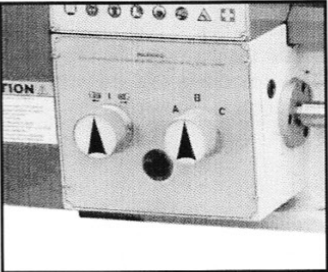
\includegraphics[width=4.6cm]{figure/asset/v4/paddle-image-0008-0003.png}};
\draw[schemaOcra,line width=1pt,line cap=round,line join=round]
  ([xshift=-3pt,yshift=-9pt]crop.north west) -- ([xshift=-3pt,yshift=3pt]crop.north west) -- ([xshift=9pt,yshift=3pt]crop.north west)
  ([xshift=-9pt,yshift=3pt]crop.north east) -- ([xshift=3pt,yshift=3pt]crop.north east) -- ([xshift=3pt,yshift=-9pt]crop.north east)
  ([xshift=-3pt,yshift=9pt]crop.south west) -- ([xshift=-3pt,yshift=-3pt]crop.south west) -- ([xshift=9pt,yshift=-3pt]crop.south west)
  ([xshift=-9pt,yshift=-3pt]crop.south east) -- ([xshift=3pt,yshift=-3pt]crop.south east) -- ([xshift=3pt,yshift=9pt]crop.south east);
\draw[schemaOcra,line width=1.1pt] (7.4,-2.65) circle (0.28);
\draw[schemaOcra,line width=1.8pt,line cap=round] (7.6,-2.85) -- (7.92,-3.17);
\draw[schema freccia,draw=schemaOcra] ({1761/400},{-1.15-1188/400}) -- (7.4,{-1.15-1188/400}) |- (crop.west);
\node[schema nota] at (11.5,-5.85) {Ritaglio: $328\times272$ pixel};
\node[schema blocco,text width=6.2cm,minimum height=1.9cm] at (3.5,-7.5)
  {\textbf{Regola geometrica}\\$\rho=\dfrac{328\cdot272}{2600\cdot1950}\simeq1{,}76\%$\\Inferiore alla soglia del $2\%$};
\node[schema esterno,text width=6.2cm,minimum height=1.9cm] at (11.5,-7.5)
  {\textbf{Conseguenza osservata}\\Nessuna chiamata al VLM\\Asset conservato, escluso dall'uso\\Comandi e simboli restano visibili};
\end{tikzpicture}
\caption{Filtro geometrico su \texttt{paddle-image-0008-0003}: a sinistra la posizione registrata in \texttt{manual.json}, a destra il ritaglio originale. L'immagine è esclusa prima della generazione, non per un errore del modello.}
\label{fig:crop-escluso-wm250}
\end{figure}

Il caso mostra il costo informativo della riduzione delle chiamate e l'utilità della conservazione degli scarti per valutarlo. L'effetto complessivo di un'eventuale eliminazione della soglia resta da verificare: la regola funziona come politica operativa, non come classificatore semantico validato.

\subsection{Tabelle: risultati storici e limite del campione finale}

Per lo schema 1.1 la matrice di accettazione riporta, in ciascuno dei due PDF digitali completi, 267 tabelle: 263 con serializzazione \texttt{structured}, quattro \texttt{unavailable} e nessuna in fallback, per 2341 righe serializzate. Le quattro indisponibilità corrispondono agli stessi elementi delle due varianti del manuale, per i quali Docling non aveva prodotto testo tabellare. Il ritaglio rimane disponibile, ma la serializzazione non ricostruisce celle assenti nell'estrazione.

Nel WM250 completo la matrice documenta dieci tabelle, nove strutturate e una indisponibile, per 289 righe. L'indisponibilità riguarda la pagina 32. Le selezioni digitali delle pagine 3 e 1004 documentano inoltre due tabelle strutturate e sei righe, inclusa la tabella degli allarmi EX1100--EX1104. Questi dati provengono dalle prove storiche, non dai due bundle V4.\footnote{\path{tesi-di-nardo/docs/acceptance-matrix.md}, sezione ``Chiusura dello schema 1.1'' e tabella dei run con prefisso \texttt{case1-schema11}, \texttt{case2-schema11} e \texttt{case3-schema11}.}

La distinzione fra output strutturato e testo indisponibile è un risultato utile della rappresentazione: il consumatore non riceve tutti i casi come se fossero tabelle complete. Non è invece dimostrata l'accuratezza di ogni cella o relazione intestazione--valore. Le caption tabellari riportate nelle vecchie selezioni appartengono al setup storico; nel workflow finale le tabelle sono serializzate senza essere inviate al VLM. Poiché le selezioni V4 contengono zero elementi \texttt{table}, non forniscono una nuova misura empirica di qualità tabellare.

\section{Esiti dell'arricchimento multimodale}
\label{sec:risultati-enrichment}

\subsection{Bilancio delle richieste e delle caption}

Le 17 chiamate finali si distribuiscono in otto esiti \texttt{enriched}, cinque \texttt{review\_required} e quattro \texttt{failed}. Le otto immagini saltate prima della chiamata non appartengono a questo denominatore. La Tabella~\ref{tab:esiti-caption} conserva la distinzione tra filtraggio, generazione e ammissibilità finale.

\begin{table}[!htbp]
\centering
\caption{Bilancio V4 da \texttt{diagnostics/enrichment.json} e \texttt{manual.json}. I gruppi descrivono stadi diversi e non vanno sommati tra loro. Tutti i 25 asset restano conservati; l'ammissibilità non misura l'accuratezza semantica.}
\label{tab:esiti-caption}
\small
\begin{tabularx}{\textwidth}{@{}Xrrr@{}}
\toprule
Fase e conteggio & Digitale & Scansione & Totale \tabularnewline
\midrule
\multicolumn{4}{@{}l}{\textbf{Acquisizione e filtro: 25 immagini}} \tabularnewline
Immagini acquisite & 16 & 9 & 25 \\
Escluse dal filtro prima della chiamata & 7 & 1 & 8 \tabularnewline
Richieste al provider & 9 & 8 & 17 \\
\midrule
\multicolumn{4}{@{}l}{\textbf{Generazione: 17 richieste, tre esiti disgiunti}} \tabularnewline
\texttt{enriched}: ammissibile secondo la politica & 7 & 1 & 8 \tabularnewline
\texttt{review\_required}: da rivedere & 1 & 4 & 5 \tabularnewline
\texttt{failed}: risposta fuori contratto & 1 & 3 & 4 \tabularnewline
\midrule
\multicolumn{4}{@{}l}{\textbf{Conservazione nel documento finale}} \tabularnewline
Caption presenti (ammissibili + da rivedere) & 8 & 5 & 13 \tabularnewline
Di cui con inclusione prevista attiva & 7 & 1 & 8 \tabularnewline
\bottomrule
\end{tabularx}
\end{table}

Il rapporto otto su diciassette descrive le richieste che producono una caption ammissibile secondo la politica implementata. Non è una misura di accuratezza. Delle tredici caption presenti, cinque sono conservate per la revisione ma escluse dall'inclusione prevista; le altre otto sono ammissibili per l'uso successivo secondo la politica.

\subsection{Aggiunte supportate e informazioni già disponibili}

Nell'immagine digitale di pagina 73, \texttt{docling-image-0073-0001}, la caption nomina le fasi U, V e W con le sigle L1, L2 e L3, il riferimento QF1 e la terra di protezione PE. Queste etichette sono visibili nel ritaglio. L'output converte quindi dettagli grafici in testo esplicito, pur essendo marcato per revisione a causa della natura elettrica del contenuto.

Il guadagno informativo non coincide con l'intera descrizione: il testo di contesto già menziona cavo, interruttore QF1 e avvertenza di spegnimento. La presenza di tali informazioni nella caption non è una scoperta visuale. Il contributo osservabile è più circoscritto e riguarda la trascrizione e l'organizzazione di etichette che il contesto fornito non enumerava nello stesso modo. Il caso mostra che una descrizione esclusa per ragioni prudenziali può contenere informazioni supportate; lo stato tecnico non è un giudizio globale sul suo contenuto.

Nella seconda immagine OCR di pagina 10, \texttt{paddle-image-0010-0002}, la caption identifica i selettori D ed E e collega la figura all'avanzamento del carrello. Tuttavia, il prompt contiene già i paragrafi \enquote{Feed Direction Selector} e \enquote{Feed Rate Selector}. Parte della descrizione riformula pertanto la baseline testuale. Il confronto non consente di attribuire al solo canale visuale la comprensione della funzione dei comandi, né dimostra un miglioramento del loro recupero mediante ricerca.

\subsection{Errori presenti anche nelle caption accettate}

Un controesempio diretto alla coincidenza fra formato e correttezza è fornito dall'immagine \texttt{docling-image-0225-0010}. La risposta descrive una barra con \enquote{10 pulsanti quadrati neri}; nel ritaglio sono visibili dodici pulsanti. La stessa risposta coglie correttamente l'evidenziazione del primo mediante un cerchio rosa, ma il conteggio è errato. La caption, lunga 486 caratteri, riceve \texttt{enriched} e l'immagine mantiene l'inclusione prevista attiva.

La Figura~\ref{fig:errore-caption-menu} permette di confrontare il conteggio visibile con l'affermazione generata e con lo stato assegnato.

\begin{figure}[htbp]
\centering
\begin{tikzpicture}[schema base]
\node[schema titolo] at (0,0.3) {Conteggio visibile e conteggio generato};
\node[schema nota,anchor=west] at (0,-0.35) {Asset digitale originale -- pagina 225, chiamata 0004};
\node[anchor=north west,inner sep=0] at (0.3,-0.9)
  {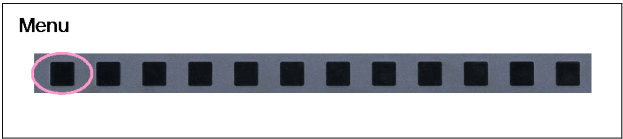
\includegraphics[width=14.4cm]{figure/asset/v4/docling-image-0225-0010.png}};
\foreach \numero/\pixel in {1/62,2/108,3/154,4/200,5/246,6/292,7/338,8/384,9/430,10/476,11/522,12/568} {
  \draw[schema icona,draw=schemaBlu!70,line width=0.5pt]
    ({0.3+14.4*\pixel/623},-4.6) -- ({0.3+14.4*\pixel/623},{-0.9-14.4*92/623});
  \node[font=\schemafont\footnotesize,text=schemaBlu] at ({0.3+14.4*\pixel/623},-4.95) {\numero};
}
\node[schema nota,text width=14cm] at (7.5,-5.55)
  {Numerazione editoriale aggiunta per rendere controllabile il conteggio: 12 pulsanti.};
\node[schema blocco,text width=6.2cm,minimum height=2cm] at (3.5,-7.35)
  {\textbf{Che cosa afferma la caption}\\[4pt]
  \enquote{10 pulsanti quadrati neri}\\[4pt]
  Il primo è descritto correttamente\\come cerchiato in rosa.};
\node[schema esterno,text width=6.2cm,minimum height=2cm] at (11.5,-7.35)
  {\textbf{Che cosa attestano i controlli}\\[4pt]
  Stato: \texttt{enriched}\\Inclusione prevista: attiva\\Formato accettato, conteggio non verificato};
\end{tikzpicture}
\caption{La caption di \texttt{docling-image-0225-0010} conta dieci pulsanti, ma nell'immagine sono dodici: il controllo di formato non rileva l'errore. Numeri e linee sono aggiunti per il confronto; il cerchio rosa è nell'originale.}
\label{fig:errore-caption-menu}
\end{figure}

La descrizione della schermata digitale di pagina 228, \texttt{docling-image-0228-0013}, introduce invece l'espressione \enquote{posizionamento robotico}. La fonte contestuale riguarda le coordinate e i punti utente della macchina ROBOCUT e non giustifica tale qualificazione. La risposta viene esclusa per lunghezza, non perché il controllo abbia riconosciuto l'interpretazione non supportata. Il motivo tecnico del fallimento e il problema semantico osservato devono quindi essere annotati separatamente.

Questi esempi non permettono di stimare il tasso di errore dell'intero campione. Consentono però di escludere una conclusione più forte ma ingiustificata: nessuno degli stati automatici garantisce che tutti i dettagli della caption siano fedeli. Un testo formalmente corretto può includere errori insieme a osservazioni esatte.

\subsection{Omissioni e comportamento dei controlli di revisione}

Per la tavola esplosa OCR di pagina 26, \texttt{paddle-image-0026-0001}, la risposta si concentra su categorie generiche quali ingranaggi, cuscinetti e trasmissione. Non riproduce le associazioni fra i numerosi riferimenti numerati e le parti; una descrizione così sintetica non sostituisce la tavola quando occorre identificare un componente specifico. Il limite di otto elementi nel prompt è compatibile con questa compressione, ma una sola esecuzione non consente di attribuirgli causalmente tutte le omissioni.

La caption classifica l'immagine come \enquote{schema/diagramma} e menziona un \enquote{motore elettrico}. La diagnostica richiede revisione per schema elettrico. Il comportamento è coerente con la regola lessicale implementata, che cerca termini elettrici nei campi descrittivi di un diagramma; non dimostra però che la tavola sia uno schema di cablaggio. L'asset è una rappresentazione esplosa di un gruppo meccanico. Il caso mostra come un controllo prudenziale possa intercettare un'espressione della risposta senza classificare semanticamente il documento sorgente.

Gli altri tre casi OCR da rivedere sono \texttt{paddle-image-0008-0004}, \texttt{paddle-image-0010-0003} e \texttt{paddle-image-0033-0001}. Il motivo salvato è una contraddizione tra la dichiarazione di assenza di incertezze e una lettura indicata come non possibile. Il controllo opera su formulazioni linguistiche: non verifica autonomamente se il dettaglio sia illeggibile, assente o semplicemente non pertinente. La segnalazione è quindi un invito alla revisione e può essere conservativa; non equivale a una valutazione umana già svolta.

Nel complesso, il ciclo V4 evidenzia aggiunte supportate, ripetizioni della baseline, omissioni e interpretazioni errate. Non fornisce una misura di beneficio netto dell'enrichment. Tale conclusione non nega che alcune caption siano informative: distingue l'esistenza di contributi utili dalla dimostrazione di un miglioramento complessivo e trasferibile.

\section{Esiti dei controlli, fallimenti e tracciabilità}
\label{sec:errori}

\subsection{Fallimenti delle caption senza perdita del bundle}

Tutti i quattro esiti \texttt{failed} delle richieste V4 sono associati al superamento del limite di 1200 caratteri. Le risposte restano conservate nelle evidenze del provider, ma non vengono pubblicate come caption generate nel documento. Le lunghezze riguardano il testo normalizzato, non i token o i byte HTTP. Le chiamate escluse sono D07 (1207 caratteri; eccedenza 7), S01 (1370; eccedenza 170), S02 (1360; eccedenza 160) e S04 (1210; eccedenza 10): le sigle identificano le registrazioni digitali e OCR usate nel grafico.

La Figura~\ref{fig:lunghezze-caption-v4} colloca le quattro esclusioni rispetto alle altre tredici risposte e alla soglia del contratto. Include anche le risposte non pubblicate come caption, evitando di rappresentare soltanto gli esiti conservati nel documento.

\begin{figure}[!htbp]
\centering
\begin{tikzpicture}[schema base,schema nota/.append style={font=\schemafont\footnotesize}]
\node[schema titolo] at (0,0.7) {Lunghezza delle risposte e stato assegnato};
\foreach \valore in {0,300,600,900,1200,1500} {
  \draw[draw=schemaGrigio!20,line width=0.4pt] ({3.4+0.007*\valore},-0.9) -- ({3.4+0.007*\valore},-10.65);
  \node[schema nota] at ({3.4+0.007*\valore},-11) {\valore};
}
\draw[draw=schemaOcra,dash pattern=on 4pt off 3pt,line width=1pt] (11.8,-0.65) -- (11.8,-10.65);
\node[schema nota,text=schemaOcra] at (11.8,0) {Limite: 1200};
\node[schema titolo] at (0,-1) {Digitale: 9 risposte};
\node[schema titolo] at (0,-6) {Scansione: 8 risposte};
\node[schema etichetta,anchor=east] at (3.1,-1.800) {D01 -- p. 73};
\draw[draw=schemaOcra!45,line width=0.8pt] (3.4,-1.800) -- (8.2510,-1.800);
\path[draw=schemaOcra,fill=schemaOcra!25] (8.1760,-1.875) rectangle +(0.15,0.15);
\node[schema nota,anchor=west] at (8.3810,-1.800) {693};
\node[schema etichetta,anchor=east] at (3.1,-2.260) {D02 -- p. 93};
\draw[draw=schemaVerde!45,line width=0.8pt] (3.4,-2.260) -- (9.9310,-2.260);
\fill[schemaVerde] (9.9310,-2.260) circle (0.075);
\node[schema nota,anchor=west] at (10.0610,-2.260) {933};
\node[schema etichetta,anchor=east] at (3.1,-2.720) {D03 -- p. 98};
\draw[draw=schemaVerde!45,line width=0.8pt] (3.4,-2.720) -- (8.6220,-2.720);
\fill[schemaVerde] (8.6220,-2.720) circle (0.075);
\node[schema nota,anchor=west] at (8.7520,-2.720) {746};
\node[schema etichetta,anchor=east] at (3.1,-3.180) {D04* -- p. 225};
\draw[draw=schemaVerde!45,line width=0.8pt] (3.4,-3.180) -- (6.8020,-3.180);
\fill[schemaVerde] (6.8020,-3.180) circle (0.075);
\node[schema nota,anchor=west] at (6.9320,-3.180) {486};
\node[schema etichetta,anchor=east] at (3.1,-3.640) {D05 -- p. 225};
\draw[draw=schemaVerde!45,line width=0.8pt] (3.4,-3.640) -- (9.8960,-3.640);
\fill[schemaVerde] (9.8960,-3.640) circle (0.075);
\node[schema nota,anchor=west] at (10.0260,-3.640) {928};
\node[schema etichetta,anchor=east] at (3.1,-4.100) {D06 -- p. 228};
\draw[draw=schemaVerde!45,line width=0.8pt] (3.4,-4.100) -- (8.7690,-4.100);
\fill[schemaVerde] (8.7690,-4.100) circle (0.075);
\node[schema nota,anchor=west] at (8.8990,-4.100) {767};
\node[schema etichetta,anchor=east] at (3.1,-4.560) {D07 -- p. 228};
\draw[draw=schemaGrigio!45,line width=0.8pt] (3.4,-4.560) -- (11.8490,-4.560);
\draw[draw=schemaGrigio,line width=1.2pt] (11.7740,-4.635) -- ++(0.15,0.15) (11.7740,-4.485) -- ++(0.15,-0.15);
\node[schema nota,anchor=west] at (11.9790,-4.560) {1207};
\node[schema etichetta,anchor=east] at (3.1,-5.020) {D08 -- p. 352};
\draw[draw=schemaVerde!45,line width=0.8pt] (3.4,-5.020) -- (9.8890,-5.020);
\fill[schemaVerde] (9.8890,-5.020) circle (0.075);
\node[schema nota,anchor=west] at (10.0190,-5.020) {927};
\node[schema etichetta,anchor=east] at (3.1,-5.480) {D09 -- p. 352};
\draw[draw=schemaVerde!45,line width=0.8pt] (3.4,-5.480) -- (10.2040,-5.480);
\fill[schemaVerde] (10.2040,-5.480) circle (0.075);
\node[schema nota,anchor=west] at (10.3340,-5.480) {972};
\node[schema etichetta,anchor=east] at (3.1,-6.800) {S01 -- p. 8};
\draw[draw=schemaGrigio!45,line width=0.8pt] (3.4,-6.800) -- (12.9900,-6.800);
\draw[draw=schemaGrigio,line width=1.2pt] (12.9150,-6.875) -- ++(0.15,0.15) (12.9150,-6.725) -- ++(0.15,-0.15);
\node[schema nota,anchor=west] at (13.1200,-6.800) {1370};
\node[schema etichetta,anchor=east] at (3.1,-7.260) {S02 -- p. 8};
\draw[draw=schemaGrigio!45,line width=0.8pt] (3.4,-7.260) -- (12.9200,-7.260);
\draw[draw=schemaGrigio,line width=1.2pt] (12.8450,-7.335) -- ++(0.15,0.15) (12.8450,-7.185) -- ++(0.15,-0.15);
\node[schema nota,anchor=west] at (13.0500,-7.260) {1360};
\node[schema etichetta,anchor=east] at (3.1,-7.720) {S03 -- p. 8};
\draw[draw=schemaOcra!45,line width=0.8pt] (3.4,-7.720) -- (10.4210,-7.720);
\path[draw=schemaOcra,fill=schemaOcra!25] (10.3460,-7.795) rectangle +(0.15,0.15);
\node[schema nota,anchor=west] at (10.5510,-7.720) {1003};
\node[schema etichetta,anchor=east] at (3.1,-8.180) {S04 -- p. 10};
\draw[draw=schemaGrigio!45,line width=0.8pt] (3.4,-8.180) -- (11.8700,-8.180);
\draw[draw=schemaGrigio,line width=1.2pt] (11.7950,-8.255) -- ++(0.15,0.15) (11.7950,-8.105) -- ++(0.15,-0.15);
\node[schema nota,anchor=west] at (12.0000,-8.180) {1210};
\node[schema etichetta,anchor=east] at (3.1,-8.640) {S05 -- p. 10};
\draw[draw=schemaVerde!45,line width=0.8pt] (3.4,-8.640) -- (8.4120,-8.640);
\fill[schemaVerde] (8.4120,-8.640) circle (0.075);
\node[schema nota,anchor=west] at (8.5420,-8.640) {716};
\node[schema etichetta,anchor=east] at (3.1,-9.100) {S06 -- p. 10};
\draw[draw=schemaOcra!45,line width=0.8pt] (3.4,-9.100) -- (11.0790,-9.100);
\path[draw=schemaOcra,fill=schemaOcra!25] (11.0040,-9.175) rectangle +(0.15,0.15);
\node[schema nota,anchor=east,fill=white,inner sep=1.5pt] at (10.9490,-9.100) {1097};
\node[schema etichetta,anchor=east] at (3.1,-9.560) {S07 -- p. 26};
\draw[draw=schemaOcra!45,line width=0.8pt] (3.4,-9.560) -- (7.5860,-9.560);
\path[draw=schemaOcra,fill=schemaOcra!25] (7.5110,-9.635) rectangle +(0.15,0.15);
\node[schema nota,anchor=west] at (7.7160,-9.560) {598};
\node[schema etichetta,anchor=east] at (3.1,-10.020) {S08 -- p. 33};
\draw[draw=schemaOcra!45,line width=0.8pt] (3.4,-10.020) -- (8.5170,-10.020);
\path[draw=schemaOcra,fill=schemaOcra!25] (8.4420,-10.095) rectangle +(0.15,0.15);
\node[schema nota,anchor=west] at (8.6470,-10.020) {731};
\draw[draw=schemaGrigio,line width=0.7pt] (3.4,-10.65) -- (13.9,-10.65);
\node[schema etichetta] at (8.65,-11.65) {Caratteri del testo normalizzato, non token};
\fill[schemaVerde] (0.6,-12.5) circle (0.075);
\node[schema nota,anchor=west] at (0.85,-12.5) {\texttt{enriched}};
\path[draw=schemaOcra,fill=schemaOcra!25] (5,-12.575) rectangle +(0.15,0.15);
\node[schema nota,anchor=west] at (5.3,-12.5) {\texttt{review\_required}};
\draw[draw=schemaGrigio,line width=1.2pt] (11,-12.575) -- ++(0.15,0.15) (11,-12.425) -- ++(0.15,-0.15);
\node[schema nota,anchor=west] at (11.3,-12.5) {\texttt{failed}};
\node[schema nota,text width=14.4cm] at (7.5,-13.55)
  {D/S: digitale/scansione; numero della chiamata; p.: pagina fisica del PDF.\\
  * D04 contiene il conteggio errato dei pulsanti, pur essendo sotto soglia.};
\end{tikzpicture}
\caption{Lunghezza delle 17 risposte V4, dai \protect\path{caption-response.json}, incluse le quattro escluse per lunghezza. Le otto immagini filtrate prima della generazione non compaiono. Il caso D04 è illustrato nella Figura~\ref{fig:errore-caption-menu}.}
\label{fig:lunghezze-caption-v4}
\end{figure}

Le eccedenze di sette e dieci caratteri rendono evidente la natura rigida del contratto: l'esclusione non è proporzionale alla qualità del contenuto. Non ne consegue che sia corretto troncare automaticamente le risposte o aumentare la soglia sulla base di questi soli esempi. Entrambe le modifiche cambierebbero il trattamento dell'output e richiederebbero nuove verifiche, in particolare per non perdere il campo delle incertezze.

Diversamente dall'esito V3 descritto nel diario, nel quale le caption fuori contratto avevano impedito la pubblicazione, le due run V4 mantengono gli altri risultati e pubblicano bundle sperimentali. La documentazione V3 è evidenza storica, non un'esecuzione qui ripetuta; la continuità V4 è invece osservabile negli artefatti. Il miglioramento sostenuto dai dati riguarda la gestione del fallimento locale, non un aumento dimostrato dell'accuratezza delle descrizioni.

\FloatBarrier
\subsection{Validazione e gate di promozione}

I report salvati superano tutti i 30 controlli dello schema 1.1. Le ragioni che impediscono lo stato \texttt{validated} sono leggibili separatamente nella diagnostica di promozione, riportata nella Tabella~\ref{tab:gate-v4}.

\begin{table}[!htbp]
\centering
\caption{Gate di promozione da \texttt{diagnostics/promotion.json}. ``No'' indica un requisito non soddisfatto, non necessariamente incoerenza tecnica. Il requisito sull'enrichment considera anche gli errori delle singole richieste.}
\label{tab:gate-v4}
\small
\begin{tabularx}{\textwidth}{@{}Xcc@{}}
\toprule
Requisito di promozione & Digitale & Scansione \tabularnewline
\midrule
Documento elaborato integralmente\newline{\footnotesize\texttt{document.full}} & No & No \tabularnewline
Enrichment configurato e senza errori\newline{\footnotesize\texttt{enrichment.configured}} & No & No \tabularnewline
Identità delle caption coerente\newline{\footnotesize\texttt{captions.identity}} & Sì & Sì \tabularnewline
Nessuna caption da rivedere\newline{\footnotesize\texttt{enrichment.review\_free}} & No & No \tabularnewline
Nessun avviso ostativo\newline{\footnotesize\texttt{warnings.nonconsequential}} & Sì & No \tabularnewline
Profilo accettato\newline{\footnotesize\texttt{profile.accepted}} & Sì & Sì \tabularnewline
Strategia strutturale accettata\newline{\footnotesize\texttt{structure.accepted}} & Sì & No \tabularnewline
\bottomrule
\end{tabularx}
\end{table}

Per entrambi i casi pesano la selezione parziale, i fallimenti del captioning e gli elementi da rivedere. Nel digitale gli avvisi su due corrispondenze normalizzate dei titoli non impediscono il superamento del gate sugli avvisi. Nel caso scansionato incidono anche i limiti della struttura parziale e il fallback. Il profilo OCR risulta accettato tramite l'evidenza storica registrata, ma questa accettazione non basta a promuovere una run che ne utilizza un percorso strutturale meno affidabile.

La combinazione fra report passato e stato sperimentale non è contraddittoria. Il report conferma che lo stato e gli artefatti rispettano il contratto e la politica; non afferma che tutti i gate di promozione siano superati. L'errore di conteggio della Figura~\ref{fig:errore-caption-menu} mostra inoltre che neppure il superamento dei controlli della singola caption coincide con la correttezza semantica.

\subsection{Integrità degli artefatti e identificazione della revisione}

L'audit descritto nella Sezione~\ref{sec:audit-metodi} conferma la corrispondenza delle fingerprint dei due bundle con i valori salvati. I digest iniziano rispettivamente con \texttt{395963bbb6ba} e \texttt{b8827d3573df}; i valori completi rimangono nei report. Risultano coerenti anche gli hash degli asset inviati, i prompt salvati e le risposte HTTP rispetto al testo normalizzato conservato nelle evidenze. Le tredici caption presenti nel documento hanno un hash di ingresso ricostruibile dagli asset e dalle richieste.

Questa catena rende controllabili anche gli esiti esclusi: è possibile distinguere un asset mai inviato, una risposta generata ma fuori contratto e una caption conservata soltanto per revisione. I contatori del report possono essere confrontati con le chiamate individuali. L'uguaglianza fra snapshot dopo l'enrichment e documento finale, in questi campioni privi di tabelle, conferma inoltre che il contenuto generativo valutato è quello effettivamente pubblicato.

Resta una limitazione dell'identità software: 32 dei 34 sorgenti registrati per ciascuna run corrispondono ai file conservati nell'archivio del progetto, mentre \texttt{enrichment.py} e \texttt{orchestrator.py} hanno hash diversi. Mancano anche lo script di strumentazione e alcuni materiali del protocollo. L'audit conferma dunque l'integrità dei bundle rispetto alle loro impronte; per la riproduzione esatta delle run occorre invece recuperare la revisione eseguita e i materiali mancanti. La verifica si limita agli artefatti conservati, senza rieseguire la suite di test o la validazione completa del corpus.

\section{Discussione, limiti e trasferibilità}
\label{sec:limiti}

\subsection{Contributo dell'integrazione}

Il risultato principale è l'organizzazione di percorsi eterogenei in un workflow con contratto comune e stati espliciti. Le prove complete documentate e i bundle selettivi mostrano che struttura, testo, asset, descrizioni e tracce possono essere rappresentati senza imporre ai consumatori il formato nativo di ciascun parser. Il valore dell'integrazione risiede anche nel rendere visibili i limiti degli stadi: una tabella può essere indisponibile, una caption può fallire e una run può restare sperimentale senza essere confusa con un output corrotto.

La convergenza formale non risolve ogni problema documentale. Il caso OCR di pagina 10 dimostra che un riferimento padre valido può essere semanticamente inadeguato. La selezione di un contesto migliore per il prompt è una mitigazione locale, non una correzione dell'intero modello gerarchico. La qualità va quindi verificata anche nelle relazioni, non soltanto nella presenza degli elementi.

\subsection{Compromessi dell'enrichment e dei controlli}

Gli esempi non sostengono né l'accettazione indiscriminata delle descrizioni né il loro rifiuto complessivo. Nel medesimo ciclo si osservano trascrizioni visuali supportate, informazioni già presenti nel contesto, conteggi errati e descrizioni troppo generiche. I controlli intercettano vincoli di formato e segnali linguistici, ma possono lasciare passare errori semantici o inviare a revisione casi che richiedono un'interpretazione più fine della fonte.

Anche le esclusioni hanno un costo. Il ritaglio WM250 sotto soglia contiene comandi riconoscibili; alcune risposte vengono scartate per un'eccedenza minima di lunghezza; le descrizioni elettriche restano escluse pur potendo contenere etichette corrette. La trasparenza di questi esiti consente di valutare il compromesso scelto fra copertura e prudenza, la cui ottimalità resta da verificare.

La separazione finale fra immagini al VLM e tabelle serializzate riduce le occasioni di riscrittura generativa dei dati tabellari. Non rende però automaticamente corrette le celle acquisite. La fedeltà del parser e quella della trasformazione successiva restano due problemi distinti, da valutare con riferimenti appropriati.

\subsection{Validità e generalizzazione}

Il corpus comprende due manuali di base e tre condizioni di ingresso; le due varianti digitali non sono indipendenti. La selezione di 17 immagini deriva dal percorso di sviluppo della pipeline, non da un campione esterno o casuale. Lo studio non comprende repliche delle generazioni o un'annotazione indipendente completa; inoltre, i PDF integrali sono assenti dall'archivio del progetto. Questi limiti impediscono di stimare generalizzazione, variabilità o tassi semantici globali con un significato statistico fondato.

Il confronto tra digitale e scansione è inoltre confuso da differenze di documento, lingua, layout e struttura disponibile. Il maggiore numero di esclusioni successive alla generazione nel caso OCR non isola l'effetto del parser o della qualità dell'immagine. Analogamente, le metriche storiche della TOC e i conteggi delle tabelle non sostituiscono l'analisi diretta delle corrispondenze o delle celle.

Infine, non sono stati misurati retrieval, qualità delle risposte dell'assistente o prestazioni degli operatori dopo l'introduzione di questa pipeline. La presenza di testo visuale aggiuntivo è una condizione che può essere sfruttata a valle, non una prova di efficacia. Le conclusioni sostenute dal lavoro riguardano l'integrazione dell'ingestion, l'ispezionabilità degli esiti e i limiti emersi nella rappresentazione e nell'enrichment.